% Adapted from "Resume Template by Krishna Priyatham Potluri"
% (Overleaf, CC BY 4.0). Content and local class customized for Sieun Park.
\documentclass{resume}

\begin{document}

\noindent
\begin{tabularx}{\linewidth}{@{}X >{\raggedleft\arraybackslash}m{2.85cm}@{}}
  {%
    {\LARGE\bfseries Sieun Park}\par
    \vspace{0.25em}
    {\large Mobile Systems Researcher}\par
    \vspace{0.15em}
    {\small \kw{Mobile \& XR AI Privacy} \textbar{} \kw{User-Configurable Privacy Control}}\par
    \vspace{0.55em}
    {\small\color{muted}\raggedright
      \contactitem{\faMapMarker*}{Seoul, South Korea}\hspace{1.2em}
      \contactitem{\faEnvelope[regular]}{\href{mailto:sieun.park@hcs.snu.ac.kr}{sieun.park@hcs.snu.ac.kr}}\ifdefined\cvnophoto\hspace{1.2em}\else\par\fi
      \contactitem{\faLink}{\href{https://cherry-0.github.io/sieunpark-at-snu/}{cherry-0.github.io/sieunpark-at-snu}}\hspace{1.2em}
      \contactitem{\faLinkedin}{\href{https://www.linkedin.com/in/sieun-park-at-snu}{sieun-park-at-snu}}\par
    }
  }
  & 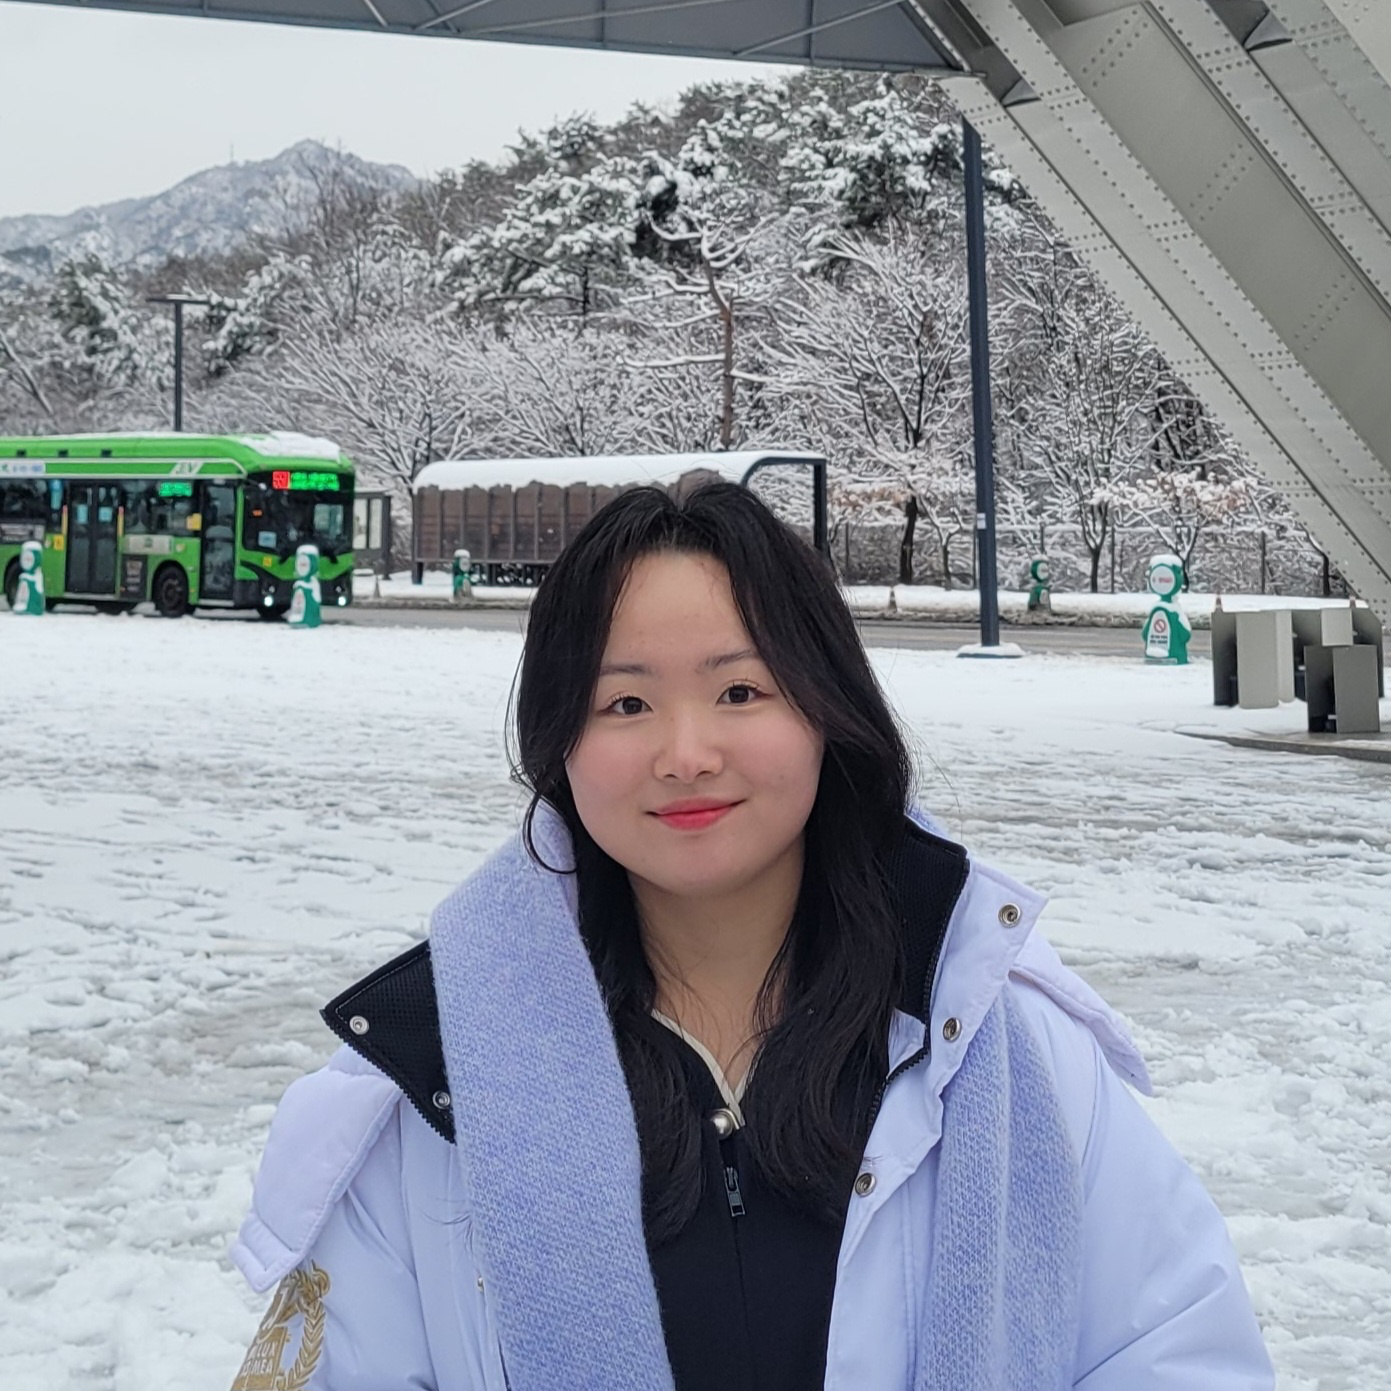
\includegraphics[width=2.8cm]{id_photo.png}
\end{tabularx}

\csection{Summary}{\small
  Mobile systems researcher studying \kw{inference-induced privacy risks} in LLM/VLM-enabled \kw{mobile and XR apps}. I trace how model-derived attributes escape input permissions and leak across app output channels, and build \kw{user-configurable privacy controls} grounded in \kw{composable privacy policies} across user, app, and system layers.
}

\csection{Education}{\small
  \resumeentry{M.S./Ph.D. in Artificial Intelligence}{Sept 2024 -- Present}{Seoul National University}{Seoul, South Korea}
  \vspace{0.35em}
  \resumeentry{B.S. in Mathematics Education \& Artificial Intelligence}{Mar 2018 -- Feb 2024}{Seoul National University}{Seoul, South Korea}
}

\csection{Research Experience}{\small
  \resumeentry{Graduate Researcher}{Sept 2024 -- Present}{Human-Centered Computer Systems Lab, Seoul National University}{Seoul, South Korea}
  \begin{itemize}
    \item XR \& Mobile Privacy
    \item User-Configurable Privacy Controls
    \item Inference-Induced Privacy Risks
    \item Privacy Policy Specification \& Composition
  \end{itemize}

}

\csection{Teaching Experience}{\small
  \resumeentry{Head Teaching Assistant, Software Development Principles and Practices}{Sept 2026 -- Dec 2026}{Seoul National University}{Seoul, South Korea}

  \vspace{0.35em}
  \resumeentry{\href{https://hcs.snu.ac.kr/course/?coursename=Software\%20Development\%20Principles\%20and\%20Practices}{Teaching Assistant, Software Development Principles and Practices}}{Sept 2025 -- Dec 2025}{Seoul National University}{Seoul, South Korea}
  \begin{itemize}[before=\fontsize{8pt}{9.5pt}\selectfont]
    \item Supported programming assignments, code reviews, and team-based software projects.
  \end{itemize}

  \vspace{0.25em}
  \resumeentry{Teaching Assistant, Education and Artificial Intelligence}{Mar 2023 -- Jun 2023}{Seoul National University}{Seoul, South Korea}
  \begin{itemize}[before=\fontsize{8pt}{9.5pt}\selectfont]
    \item Mentored project teams designing AI-driven educational applications and provided feedback on technical implementation and pedagogical grounding.
  \end{itemize}
}

\csection{Publications}{\small
  \publicationentry
    {TaleTrain: AI Scaffolding for Parent--Child Video Story Retelling at Home}
    {Sangwon Park, \textbf{Sieun Park}, HyunA Seo, Minkyu Shim, Youngki Lee}
    {Under Review}
  \vspace{0.35em}
  \publicationentry
    {ODFuse: Reducing Reasoning Overhead in Tool-Use Agents via Observation-Dependency-Guided Fusion}
    {Hyunwoo Jung, \textbf{Sieun Park}, Minkyu Shim, Youngki Lee}
    {Under Review}
}

\csection{Presentations}{\small
  \presentationentry
    {\href{https://cherry-0.github.io/sieunpark-at-snu/presentations/mobisys-26/}{Governing Hidden Inference: Output-Centric Privacy Control for AI Apps}}
    {ACM MobiSys 2026}
  \vspace{0.35em}
  \presentationentry
    {\href{https://cherry-0.github.io/sieunpark-at-snu/presentations/stop-the-hidden-inference/}{Stop the Hidden Inference: Privacy Safeguards Beyond Permissions}}
    {UIST 2025 Workshop \textperiodcentered{} Poster}
  \vspace{0.35em}
  \presentationentry
    {\href{https://cherry-0.github.io/sieunpark-at-snu/presentations/at-your-fingertips/}{At Your Fingertips: On-Demand Affordances for Cross-Spatial Object Interaction}}
    {CHI 2025 Workshop}
}

\csection{Research Areas \& Languages}{\small
  \textbf{Research Areas:} Mobile AI Privacy, Accountable Mobile Systems, HCI\par
  \vspace{0.2em}
  \textbf{Languages:} Korean (native), English (professional working proficiency)
}

\end{document}
